\documentclass{boi2014-lv}

\usepackage{enumitem}
\usepackage{todonotes}

\renewcommand{\DayNum}{0}
\renewcommand{\TaskCode}{network}
\renewcommand{\TaskName}{Datortīkls}

\begin{document}
    
		Skolas datorklasē ir $N$ datori, kas savā starpā savienoti ar tīkla vadiem. Katrs tīkla
		vads savieno divus dažādus datorus. Zināms ka jebkuriem diviem datoriem izpildās šāda īpašība, ja  
		datori savā starpā nav savienoti pa tiešo ar vadu, tad vienmēr ziņojumus iespējams nosūtīt  
		izmantojot citus ar tīkla vadiem savienotos datorus, tos lietojot kā starpniekiem.
		Ziņojums vienmēr tiek sūtīts pa īsāko ceļu: tā lai ziņojums nonāktu pēc iespējas mazāk \emph{starpniekdatoros} 
		(tajos datoros, kas nav ne ziņas sūtītājs, ne saņēmējs).
				
		%There are $N$ computers in the computer classroom of a local secondary
    %school and they are connected with cables to form a single network. Each
    %cable joins two distinct computers.  Some pairs of computers may not be
    %joined by a cable directly, but a message can always be sent from any
    %computer to any other computer through intermediate computers joined by
    %cables.  A message always chooses the shortest route to travel: the number
    %of \emph{intermediate computers} along its path (i.e. computers other than
    %sender and receiver that the message visits) is minimised.
    
		Ādams un Billijs, kas lieto atšķirīgus datorklases datorus $a$ un $b$, vēlas noskaidrot
		īsāko ceļu starp viņu datoriem. Viņi nezina tīkla vadu izvietojumu, bet viņi var sūtīt
		ziņojumus starp jebkuriem diviem datorklases datoriem un noskaidrot apmeklēto starpniekdatoru
		skaitu.
    
		%Adam and Billy, who use distinct computers $a$ and $b$ in this classroom,
    %wish to determine a shortest route between their computers. They do not
    %know the layout of the cables but they can send messages between all pairs
    %of computers and calculate the number of intermediate computers that they
    %visit.

		Ādams un Billijs nav draugos ar datoru tāpēc viņi lūdz tevi palīgā noskaidrot īsāko ceļu starp
		viņu datoriem sūtot pēc iespējas maz ziņojumu.
    %However, Adam and Billy are not very good with computers
    %and they ask you for help to achieve their goal without sending
    %too many messages.

    \Task
		
		Atrodiet īsāko ceļu starp datoriem $a$ un $b$ nepārsniedzot atļauto ziņojumu sūtījumu skaitu.
		
    %Find a shortest route between computers $a$ and $b$ without
    %sending more messages than is allowed.

    \Implementation
		Jums jāimplementē procedūra \method{findRoute(N, a, b)} ar šādiem parametriem:
    %You need to implement one procedure \method{findRoute(N, a, b)} that
    %takes the following parameters:

    \begin{itemize}
        \item $N$ --- datoru skaits datorklasē
            (tie ir sanumurēti ar skaitļiem no $1$ līdz $N$)
        \item $a, b$ --- Ādama un Billija datoru numuri
            ($a \neq b$ un $1 \le a, b \le N$)
    \end{itemize}

		Jūsu procedūra \method{findRoute} var izsaukt funkciju \method{ping(i, j)},
		kas kā parametrus saņem divu dažādu datoru numurus ($i \neq j$ un $1 \le i, j \le N$)
		un atgriež starpniekdatoru skaitu, kas tika izmantots, lai nosūtītu ziņojumu no datora
		$i$ uz $j$.
    %Your procedure \method{findRoute} can call function \method{ping(i, j)}
    %that takes as parameters labels of two distinct computers
    %($i \neq j$ and $1 \le i, j \le N$) and returns the number of intermediate computers
    %that a message travelling from $i$ to $j$ would visit.

		Jūsu procedūrai \method{findRoute} jāapraksta īsākais ceļš, pa kuru varētu tikt sūtīts 
		ziņojums no $a$ uz $b$. Īsākā ceļa aprakstīšana jāveic atkārtoti izsaucot procedūru
		\method{travelTo(k)}, kas parametrā saņem tā datora numuru, kas saņems ziņojumu kā nākamais ($1 \le k \le N$).
		Ziņojums sākumā atrodas datorā $a$, kad tiek izsaukta metode \method{travelTo(k)} ziņojums tiek pārsūtīts uz datoru $k$.
    %Your procedure \method{findRoute} has to describe a shortest route
    %that a message sent from $a$ to $b$ might take. This must be done by
    %repeatedly calling procedure \method{travelTo(k)} that takes as
    %parameter the label of computer to which the message should travel
    %next ($1 \le k \le N$). The message starts at $a$, and whenever
    %\method{travelTo(k)} is called, it moves to computer $k$.

		Papildus pamatnosacījumiem (laika un atmiņas ierobežojumiem, 
		darbība bez izpildlaika kļūdām) Jūsu iesūtītajam risinājumam, lai tas tiktu ieskaitīts, 
		jāievēro šādi nosacījumi:
    %In addition to the standard requirements (time and memory
    %limits, no runtime errors), your submission has to achieve the following
    %in order to solve a testcase:

    \begin{itemize}
        \item kad \method{findRoute} beidz darbu, ziņojumam jābūt nonākušam datorā $b$,
				%\item the message must be at $b$ when procedure \method{findRoute}
        %    terminates,
        \item katriem diviem secīgiem datoriem jābūt savienotiem ar tīkla vadu,
        %\item any two consecutive computers in its path must be joined
        %    by a cable,
        \item ziņojums jāsūta pa īsāko ceļu,
				%\item it must take a shortest route,
        \item funkcijas \method{ping} izsaukumu skaits $M$ nedrīkst pārsniegt atļauto izsaukumu skaitu (skat. Vērtēšana),
        %\item the number $M$ of calls to function \method{ping} must not
        %    exceed the allowed limit (see section Scoring),
        \item funkcija \method{ping} un procedūra \method{travelTo} jāizsauc tikai ar pieļaujamām parametru vērtībām.
        %\item function \method{ping} and procedure \method{travelTo} must
        %    only be called with allowed parameter values.
    \end{itemize}

    \Example
    Par piemēru ņemsim diagrammā attēloto datoru tīklu (apļi attēlo datorus, bet līnijas --- tīkla vadus). Datortīklā 
		kopā ir $N = 4$ datori. Pieņemsim, ka Ādams un Billijs lieto datorus $a = 1$ and $b = 4$.
		
		%Consider the example shown in the diagram below (points correspond to
    %computers, lines --- to cables). There are $N = 4$ computers in total,
    %and Adam and Billy are using computers $a = 1$ and $b = 4$.

    \begin{wrapfigure}[1]{r}{5cm}
        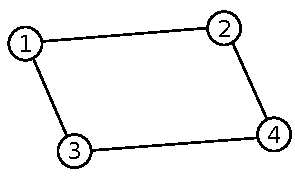
\includegraphics{network-example}
    \end{wrapfigure}

		Tiks izsaukta procedūra
    %%The first call will be to procedure
    \begin{figure}[H]
        \centering
        \method{findRoute(4, 1, 4)}.
    \end{figure}

		Šajā gadījumā tās uzvedība varētu būtu šāda:
    %Its sample behaviour could be as follows:

    \begin{figure}[H]
        \centering
        izsauc \method{ping(1, 4)}, kas atgriež vērtību $1$, \\
        izsauc \method{ping(1, 2)}, kas atgriež vērtību $0$, \\
        izsauc \method{ping(2, 4)}, kas atgriež vērtību $0$.
    \end{figure}

		Ar šo informāciju pietiek, lai noteiktu ka $1 \to 2 \to 4$ ir īsākais ceļš $1$ uz $4$. Šo ceļu var aprakstīt šādi:
    %This information is sufficient to determine that $1 \to 2 \to 4$ is a
    %shortest route from $1$ to $4$. This should be described as follows:

    \begin{figure}[H]
        \centering
        izsauc \method{travelTo(2)}, \\
        izsauc \method{travelTo(4)}, \\
        \method{findRoute} beidz darbu.
    \end{figure}

    \Scoring
    Visiem apakšuzdevumiem ir spēkā $2 \le N \le 1000$.

    \begin{description}

        \item[Apakšuzdevums 1 (25 punkti):] starp katriem diviem datoriem ir tieši viens īsākais ceļš; $M$ Nedrīkst pārsniegt $2N$.
        \item[Apakšuzdevums 2 (25 punkti):] $M$ Nedrīkst pārsniegt $N^2$.
        \item[Apakšuzdevums 3 (25 punkti):] $M$ Nedrīkst pārsniegt $4N$.
        \item[Apakšuzdevums 4 (25 punkti):] $M$ Nedrīkst pārsniegt $2N$.
    \end{description}

    \Constraints
    \begin{description}
        \item[Laika ierobežojums:] 1 s.
        \item[Atmiņas ierobežojums:] 64 MB.
    \end{description}

    \Experimentation
    Pārbaudes programma uz Jūsu datora lasīs ievaddatus no standarta ievada.
		Pirmajā ievaddatu rindā jābūt četriem veseliem skaitļiem $N, a, b$ un $M$ ierobežojumam.
		Katrā no nākamajām $N$ rindām jābūt $N$ veseliem skaitļiem, kas apraksta tīkla vadu izvietojumu:
		$i$-tās rindas $j$-tais skaitlis ($i \neq j$) norāda starpniekdatoru skaitu kādu izmantotu, ja
		sūtītu ziņu no $i$ uz $j$. Nav svarīgi kādas ir norādītās vērtības ja $i = j$.
    %The sample grader on your computer will read data from standard input.
		%The first line of input should contain four integers $N, a, b$ and the
    %allowed limit for $M$. The next $N$ lines should
    %contain $N$ integers each, describing the layout of the cables:
    %the $j$--th integer in the $i$--th of these rows ($i \neq j$) should be
    %the number of intermediate computers that a message sent from $i$ to $j$
    %would visit. It does not matter what the entries with $i = j$ are.

    %The following input describes the above example with $M$ limited by
		Šeit redzams, kā būtu aprakstīts iepriekšaplūkotais piemērs, ja $M$ ierobežots ar
    $100$:

    \begin{center}
        \begin{tabular}{p{4cm}}
            {\tt
                4 1 4 100 \newline
                0 0 0 1 \newline
                0 0 1 0 \newline
                0 1 0 0 \newline
                1 0 0 0
            }
        \end{tabular}
    \end{center}

\end{document}

